\section{Results} \label{secResults}

We present our results from each of our fits.
We used Wolfram Mathematica 9 to calibrate our models, and much of our analysis
assumes the correctness of Wolfram Mathematica 9's kernel and functions.\\
\\
This section of results is organised as follows.
Subsection \ref{subsecData} briefly gives some salient points about the data
itself, such as the mean time to complete each attempt and the standard
deviation.
Subsection \ref{subsecP1LA} shows the results of fitting our three models to
\PO\ using \LA.
Subsection \ref{subsecP1LB} shows the results of fitting our three models to
\PO\ using \LB.
Subsection \ref{subsecP2LA} shows the results of fitting our three models to
\PT\ using \LA.
Subsection \ref{subsecInd} shows individual results --- namely, my own for both
lines of code and time to show how the models may be inappropriate for
an individual's design process.

\subsection{Analysing the data} \label{subsecData}

Some basic analyses that we performed on the data are presented below.
Although they do not contribute to answering our seven questions, we can make
some further comments and possible insights into the data and its usefulness.\\
\\
First, we begin by analysing the data for \PO\ when it was completed four
separate times in \LA, as shown in table \ref{tableP1LA}.

\begin{table}[ht!]
\centering
\begin{tabular}{|c|c|c|}
\hline
{\bf Attempt} &  {\bf Mean (minutes)} & {\bf Standard Deviation (minutes)} \\
\hline
\AZ & 172.857 & 91.6195 \\
\hline
\AO & 91.2143 & 69.0698 \\
\hline
\AT & 73.7857 & 49.6343 \\
\hline
\ATh & 40.2143 & 28.722 \\
\hline
\end{tabular}
\caption{Data from the analysis of \PO\ when completed with \LA.}
\label{tableP1LA}
\end{table}

This analyses suggests that the students began with a very wide range of abilities
and domain knowledge about the problem.
We can see what they began with needing almost 3 hours to finish the task, with a
standard deviation of more than 50\% of the mean.
As they continued to practice on the problem, the mean sharply decreased and the
standard deviation (approximately the spread of student times) began to contract.
However, the standard deviation as a percentage of the mean is still quite high.
This suggests that although the skill of the group as a whole was increasing, the
rates of learning, and the way that each student approached each iteration were quite
different across the entire group.\\
\\
Table \ref{tableP1LB} shows the analysis of the data for completing \PO\ in
\LB\ four times.

\begin{table}[ht!]
\centering
\begin{tabular}{|c|c|c|}
\hline
{\bf Attempt} &  {\bf Mean (minutes)} & {\bf Standard Deviation (minutes)} \\
\AZ & 102.643 & 40.3229 \\
\hline
\AO & 62.7143 & 38.0777 \\
\hline
\AT & 50.1429  & 30.1046 \\
\hline
\ATh & 43.5714 & 27.2134\\
\hline
\end{tabular}
\caption{Data from the analysis of \PO\ when completed with \LB.}
\label{tableP1LB}
\end{table}

We can immediately see that the students were much faster in their first attempt for
\PO\ in \LB.
We will compare their differences more in section \ref{secAnalysis}.
It is worth noting that the spread of times is much smaller and the mean times are lower.
However, we also note that subsequent attempts did not show as much improvement as in the
first set of data.
The mean of their final times was comparable to the mean time taken for the final attempt
of \PO\ in \LA, but the spread has dramatically decreased.
This suggests that the students' skills and knowledge were converging and suggests this
dataset was much more reliable.\\
\\
Table \ref{tableP2LA} shows the analysis of the data for completing \PT\ in
\LA\ four times.

\begin{table}[ht!]
\centering
\begin{tabular}{|c|c|c|}
\hline
{\bf Attempt} &  {\bf Mean (minutes)} & {\bf Standard Deviation (minutes)} \\
\hline
\AZ & 100.143 & 70.1415 \\
\hline
\AO & 54.2143 & 38.573 \\
\hline
\AT & 49.9286  & 38.8794 \\
\hline
\ATh & 39.1429 & 34.9436\\
\hline
\end{tabular}
\caption{Data from the analysis of \PT\ when completed with \LA.}
\label{tableP2LA}
\end{table}

This dataset suggests that the knowledge from the previous problem domain transferred
over to the new dataset quite well.
The average time required to complete the problem was lower, but the spread of times was much higher.
The spread also did not converge as readily or tightly as the previous dataset.
We note that the differences in times between each dataset were far more erratic.
This suggests that language and resource changes are easier to deal with than problem domain
changes.

\subsection{Problem one in language A} \label{subsecP1LA}

We first present our results for \PO\ in \LA.
Table \ref{table:P1LA:abc} shows our best fit parameters.
Table \ref{table:P1LA:abc:error} gives the standard errors for each of the
parameter estimates.
Table \ref{table:P1LA:abc:sumsquares} is the sum of squares of the residuals of
the model against the data, giving us a rough idea of how good the fit was.\\
\\
Before showing the data, a brief comment about the models.
This is the only dataset where models $m_1$ and $m_2$ were unable to give
sensible results.
This is also the dataset with the greatest change in times from \AZ\ to \ATh.
We conjecture without proof or evidence that models $m_1$ and $m_2$ are not
tolerant to substantial increases in knowledge (and implicitly greatly reduced
time taken in each attempt).

\begin{table}[ht!]
\centering
\begin{tabular}{|c|c|c|c|}
\hline
{\bf Model} &  $a$ & $b$ & $c$ \\
\hline
$m_1$ & 172.652 & 0.712 & -19.8246 \\
\hline
constrained $m_1$ & 172.931 & 281.107 & 64.8165 \\
\hline
$m_2$ & 172.607 & 0.638207 & -49.9154\\
\hline
constrained $m_2$ & 172.857 & $1.67721 \times 10^10$ & 65.0713 \\
\hline
$m_3$ & 172.322 & 0.794716 & 29.691 \\
\hline
\end{tabular}
\caption{Parameters of the best fits for each of the models for \PO\ in \LA.}
\label{table:P1LA:abc}
\end{table}

During the modelling process, $m_1$ and $m_2$ both found negative $c$ values to
give the best fit.
This is quite troubling --- it suggests that these models are both inappropriate
for use in modelling learning.
The constrained $m_1$ and $m_2$ models have the additional constraints given in
Equations \ref{conThree} and \ref{conFour}, that is
\[
  a > c > 0
\]
and
\[
  b > 0.
\]

\begin{figure}[ht!]
\centering
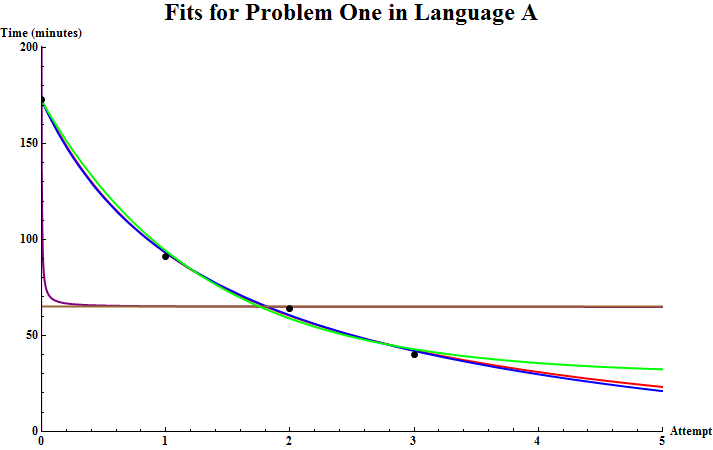
\includegraphics[scale=0.35,angle=90]{./media/P1LAGraph.png}
\caption{The graph of models for \PO\ in \LA. The key is as follows:
		 red is $m_1$,
		 purple is $m_1$, constrained explicitly with conditions \ref{conThree} and \ref{conFour},
		 blue is $m_2$,
		 brown is $m_2$, constrained explicitly with conditions \ref{conThree} and \ref{conFour},
		 green is $m_3$.
}
\label{figure:P1LA:abc}
\end{figure}

Adding these constraints in did not result in a good fit --- Mathematica
returned that the fit did not converge and gave nonsensical values for $b$ (that
is the learning rate).
This suggests that both $m_1$ and $m_2$ are inappropriate for modelling repeated
iterations of a task.
$m_3$ finds a more suitable fit which suggests that it was more robust in
finding sensible fits.
A final comment is that the $a$ values are all very similar and have negligible
differences between them, suggesting that the $a$ values are relatively similar.
More information might be found by examining the confidence for each of the
parameter fits that Mathematica found.

\begin{table}[ht!]
\centering
\begin{tabular}{|c|c|c|c|}
\hline
{\bf Model} &  $a$ & $b$ & $c$ \\
\hline
$m_1$ & 4.51941 & 0.18701 & 19.8109 \\
\hline
constrained $m_1$ & 35.9144 & 53906.8 & 49.4857 \\
\hline
$m_2$ & 4.1785 & 0.236003 & 54.71152\\
\hline
constrained $m_2$ & N/A & N/A & N/A \\
\hline
$m_3$ & 6.34312 & 0.189644 & 13.1391 \\
\hline
\end{tabular}
\caption{Standard error on the parameters of the best fits for each of the models for \PO\ in \LA.
Note that when calculating the standard errors for the constrained $m_2$ the
  computer repetitively crashed and so these values are not included.}
\label{table:P1LA:abc:error}
\end{table}

We take the standard errors for each of the parameters from each of the fits that Mathematica yielded.
Notice that while the $a$ parameters have low errors, the errors for $c$ and $b$ are
much greater (indeed, they are significant percentages of the parameters $c$ and
$b$ --- as an example, giving a confidence interval of approximately $\pm
23.78\%$ for the $b$-value of $m_3$).
Even more interesting are the standard errors for $b$ in the constrained $m_1$
and $m_2$.
This is a ridiculous
figure in the constrained $m_1$ and it unfortunately crashed Mathematica (and my
computer) when calculating the errors for the constrained $m_2$.
This suggests that these models did not fit very well to the data given, and
that although our value for $a$ is relatively accurate our value for $c$ is
quite inaccurate.

\begin{table}[ht!]
\centering
\begin{tabular}{|c|c|}
\hline
{\bf Model} & Sum of squares \\
\hline
$m_1$ & 20.4672649169\\
\hline
constrained $m_1$ & 1290.3821781171\\
\hline
$m_2$ & 17.5223504018\\
\hline
constrained $m_2$ & 1302.9796653729\\
\hline
$m_3$ & 40.5502881745 \\
\hline
\end{tabular}
\caption{Sum of squares of the residuals for the best fits for each of the models for \PO\ in \LA.}
\label{table:P1LA:abc:sumsquares}
\end{table}

It is most interesting to note that although the constrained $m_1$ and $m_2$ did
not fit well (and hence we ought to disregard them),
the unconstrained models $m_1$ and $m_2$ had very low sums of
squares compared to $m_3$ --- this suggests that perhaps they could fit the data
very well, but not in a sensible manner.
This seems to support the conjecture that they are not tolerant to such high
learning rates and will give nonsensical results.

\subsection{Problem one in language B} \label{subsecP1LB}

We now present our results for \PO\ in \LB.
Table \ref{table:P1LB:abc} shows our best fit parameters.
Table \ref{table:P1LB:abc:error} gives the standard errors for each of the
parameter estimates.
Table \ref{table:P1LB:abc:sumsquares} is the sum of squares of the residuals of
the model against the data, giving us a rough idea of how good the fit was.

\begin{table}[ht!]
\centering
\begin{tabular}{|c|c|c|c|}
\hline
{\bf Model} &  $a$ & $b$ & $c$ \\
\hline
$m_1$ & 103.736 & 1.05646 & 25.0618 \\
\hline
$m_2$ & 102.633 & 1.05789 & 25.9886\\
\hline
$m_3$ & 102.57 & 1.03095 & 41.3707 \\
\hline
\end{tabular}
\caption{Parameters of the best fits for each of the models for \PO\ in \LB.}
\label{table:P1LB:abc}
\end{table}

\begin{figure}[ht!]
\centering
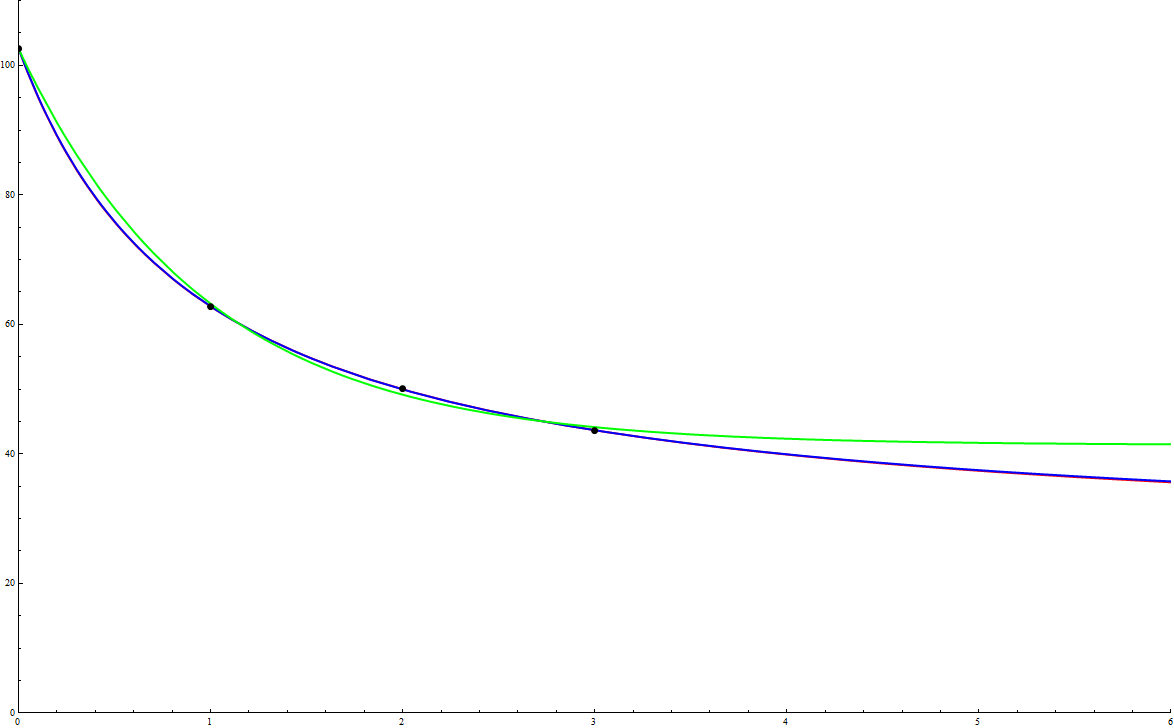
\includegraphics[scale=0.35,angle=90]{./media/P1LBGraph.png}
\caption{The graph of models for \PO\ in \LB. The key is as follows:
		 red is $m_1$,
		 blue is $m_2$,
		 green is $m_3$.
}
	\label{figure:P1LB:abc}
\end{figure}

Notice again that the $a$ values are relatively similar.
This time, the $b$ values are also quite close, and the $c$ values are the only
real differences in the models.
Each of these models gave sensible results, which suggests that since the
learning rate between each iteration seemed lower compared attempts in \PO\ in
\LB, the model is able to give useful and meaningful results.

\begin{table}[ht!]
\centering
\begin{tabular}{|c|c|c|c|}
\hline
{\bf Model} &  $a$ & $b$ & $c$ \\
\hline
$m_1$ & 0.200046 & 0.0268934 & 0.635585 \\
\hline
$m_2$ & 0.224989 & 0.0312964 & 1.17134\\
\hline
$m_3$ & 1.24103 & 0.0954955 & 1.80347 \\
\hline
\end{tabular}
\caption{Standard errors for the parameters of the best fits for each of the models for \PO\ in \LB.}
\label{table:P1LB:abc:error}
\end{table}

The errors in Table \ref{table:P1LB:abc:error} are minuscule in comparison to
Table \ref{table:P1LA:abc:error}.
Notice that $m_1$ had the smallest errors, whilst $m_3$ had consistently higher
errors than $m_1$ or $m_2$.
This suggests that $m_3$ might be more tolerant to high learning rates, but
gives a poorer fit overall.

\begin{table}[ht!]
\centering
\begin{tabular}{|c|c|}
\hline
{\bf Model} & Sum of squares \\
\hline
$m_1$ & 0.0400487707\\
\hline
$m_2$ & 0.0507152055\\
\hline
$m_3$ & 1.5429195761\\
\hline
\end{tabular}
\caption{Sum of squares of the residuals for the best fits for each of the models for \PO\ in \LB.}
\label{table:P1LB:abc:sumsquares}
\end{table}

The results of the standard errors in Table \ref{table:P1LB:abc:error} are
confirmed in Table \ref{table:P1LB:abc:sumsquares} (the sum of squares of the
residuals).
Although all models have very low sum of squares, $m_3$ has a greater sum of
squares of the residuals than $m_1$ and $m_2$.
Furthermore, $m_1$ again had the lowest sum of squares (and as shown in Table
\ref{table:P1LB:abc:error} the lowest errors for the parameters) which suggests
that here, it was the best fit.

\subsection{Problem two in language A} \label{subsecP2LA}

We now present our results for \PO\ in \LB.
Table \ref{table:P2LA:abc} shows our best fit parameters.
Table \ref{table:P2LA:abc:error} gives the standard errors for each of the
parameter estimates.
Table \ref{table:P2LA:abc:sumsquares} is the sum of squares of the residuals of
the model against the data, giving us a rough idea of how good the fit was.

\begin{table}[ht!]
\centering
\begin{tabular}{|c|c|c|c|}
\hline
{\bf Model} &  $a$ & $b$ & $c$ \\
\hline
$m_1$ & 100.079 & 1.78221 & 30.7798 \\
\hline
$m_2$ & 100 & 1.62075 & 34.7768\\
\hline
$m_3$ & 99.9429 & 1.39094 & 41.4713 \\
\hline
\end{tabular}
\caption{Parameters of the best fits for each of the models for \PT\ in \LA.}
\label{table:P2LA:abc}
\end{table}

\begin{figure}[ht!]
\centering
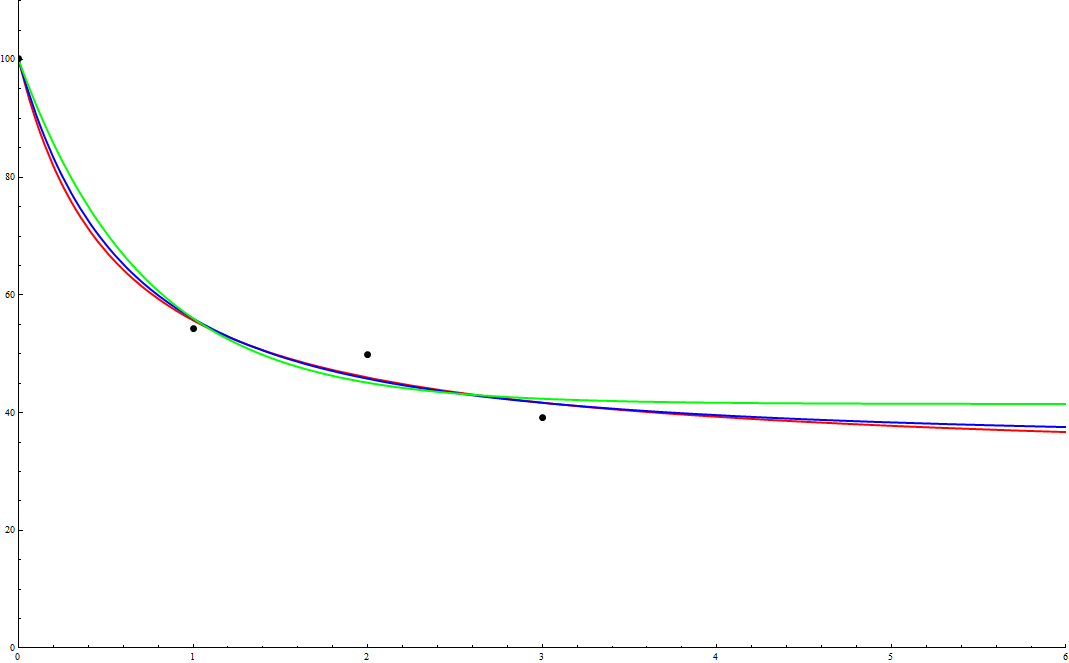
\includegraphics[scale=0.35,angle=90]{./media/P2LAGraph.png}
\caption{The graph of models for \PT\ in \LA. The key is as follows:
		 red is $m_1$,
		 blue is $m_2$,
		 green is $m_3$.
}
	\label{figure:P2LA:abc}
\end{figure}

Again, as in Table \ref{table:P1LA:abc} and \ref{table:P1LB:abc} we note that
the $a$ values as shown in Table \ref{table:P2LA:abc} are very similar.
The $b$ values show much more difference than in Table \ref{table:P1LB:abc}, and
the $c$ values show a reasonable variation (this is by inspection only, and
without justification through evidence).

\begin{table}[ht!]
\centering
\begin{tabular}{|c|c|c|c|}
\hline
{\bf Model} &  $a$ & $b$ & $c$ \\
\hline
$m_1$ & 4.94326 & 1.25419 & 11.5227 \\
\hline
$m_2$ & 5.18028 & 0.883591 & 13.2946 \\
\hline
$m_3$ & 6.08996 & 0.662606 & 6.49302 \\
\hline
\end{tabular}
\caption{Standard errors for the parameters of the best fits for each of the models for \PT\ in \LA.}
\label{table:P2LA:abc:error}
\end{table}

Table \ref{table:P2LA:abc:error} shows some interesting results.
First, we see that the $a$ values have similar errors that are quite small,
whilst the $b$ values have significant errors, suggesting confidence intervals
that can be as high as $\pm 70.372\%$ (for the $b$ value of model $m_1$).
Secondly, we note that the $c$ values had high errors in all models except $m_3$
--- indeed, $m_3$ had extremely low errors for the $b$ and $c$ values.
We ought to note that in Table \ref{tableP2LA} the differences between the means
of each attempt are quite extreme and perhaps are not as amenable to analysis.

\begin{table}[ht!]
\centering
\begin{tabular}{|c|c|}
\hline
{\bf Model} & Sum of squares \\
\hline
$m_1$ & 24.439796138\\
\hline
$m_2$ & 26.8556022611\\
\hline
$m_3$ & 37.098573229\\
\hline
\end{tabular}
\caption{Sum of squares of the residuals for the best fits for each of the models for \PT\ in \LA.}
\label{table:P2LA:abc:sumsquares}
\end{table}

The sum of squares of residuals as shown in Table \ref{table:P2LA:abc:sumsquares}
supports our suggestions that this dataset was not as amenable to analysis.
Again we see that $m_1$ had the lowest sum of squares, which suggests it was the
best fit.\\
\\
From our data, we would suggest that $m_1$ would give the best fits from our analysis of \PT\
in \LA\ and \PO\ in \LB.
However, the useless results it gives in analysing the dataset for \PO\ in \LA\
suggests that it is not tolerant to extremely high learning rates and should be
used with care.
We also note that $m_3$ will consistently give good and useful results but will
not fit as well as $m_1$, though it is a good alternative when the $m_1$ gives
bad results.
Since we have so few data points, it is a very rudimentary and early analysis
and we note that our results are still not very reliable.
We will next try using our models $m_1$, $m_2$ and $m_3$ to analyse my data and
a random student's data.

\subsection{Individual Data} \label{subsecInd}

In this section, we show how my own data fits the different curves.
Some comments about my design process:
\begin{itemize}
  \item I completed the task in C++
  \item in \AZ\ I attempted to adhere to good design practices, but this
  diminished as I completed more iterations of the task
  \item I used the same algorithm each time
  \item I had a Waterfall-esque design methodology
\end{itemize}

Firstly, we will fit my lines of code to the data.
\begin{itemize}
  \item Table \ref{table:LOC} gives the lines of code in a tabulated form
  \item Figure \ref{table:LOC} shows a line graph of the lines of code
  \item Table \ref{table:LOC:abc} shows the parameters of the best fits for the
  models we were given
  \item Table \ref{table:LOC:abc:error} shows the standard errors on the parameters
  for the best fits of the models we use
  \item Table \ref{table:LOC:abc:sumsquares} shows the sums of the squares of the
  residuals for the models we are given
\end{itemize}

\begin{table}[ht!]
\centering
\begin{tabular}{|c|c|c|c|c|}
\hline
Attempt & \AZ & \AO & \AT & \ATh\\
\hline
Lines of code & 224 & 114 & 98 & 98 \\
\hline
\end{tabular}
\caption{My own individual data for lines of code. Standard deviation of
  60.80296, coefficient of variation of 0.455453 and mean of 133.5 lines of
    code.}
\label{table:LOC}
\end{table}

\begin{figure}[ht!]
\centering
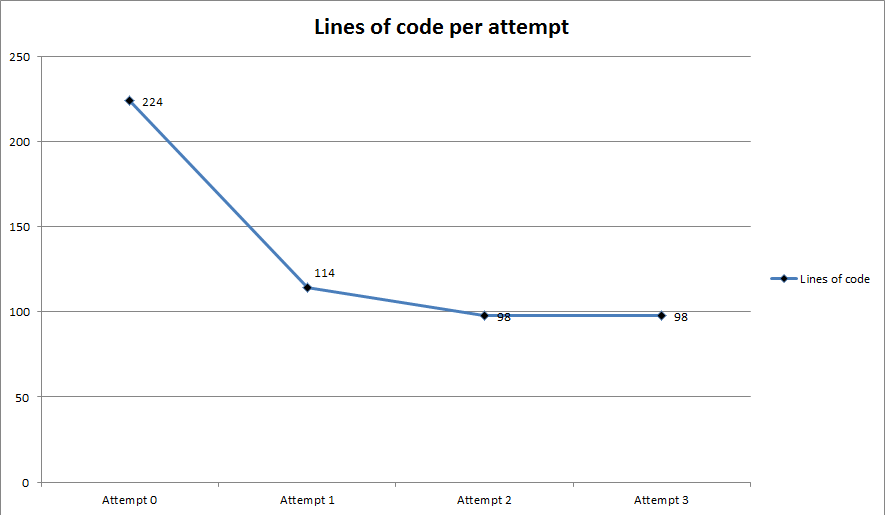
\includegraphics[scale=0.65]{./media/MyData_LOC.png}
\caption{The lines of code as a line graph --- notice that it may also be
  amenable to a similar analysis as the one we performed in the previous
    subsections.}
\label{figure:LOC}
\end{figure}

What is notable is the (almost) halving of the number of lines of code between
\AZ\ and \AO.
This is due to me cutting a lot of unnecessary code out of the solutions I used.
This will have interesting effects on the rest of my results, as we will see in
later figures.

\begin{table}[ht!]
\centering
\begin{tabular}{|c|c|c|c|}
\hline
{\bf Model} &  $a$ & $b$ & $c$ \\
\hline
$m_1$ & 224.012 & 3.99377 & 85.3736 \\
\hline
$m_2$ & 224.028 & 2.71905 & 93.5197\\
\hline
$m_3$ & 224.015 & 2.01731 & 96.8399 \\
\hline
\end{tabular}
\caption{Parameters of the best fits for each of the models for the my data's
  lines of code.}
\label{table:LOC:abc}
\end{table}

\begin{figure}[ht!]
\centering
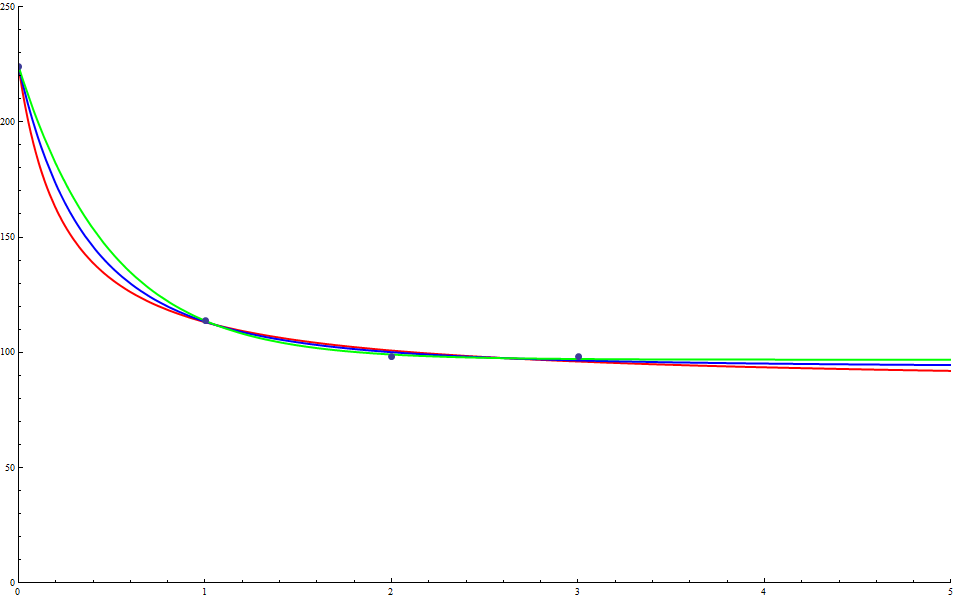
\includegraphics[scale=0.35,angle=90]{./media/LOCGraph.png}
\caption{The graph of models for the lines of code during my attempts. The key is as follows:
		 red is $m_1$,
		 blue is $m_2$,
		 green is $m_3$.
}
	\label{figure:LOC:abc}
\end{figure}

We note that each of these fits again has a similar $a$ value, but 
reasonably varying $c$ values.
The learning rate on each also changes, but at least each one has given sensible
values in this situation.
We suspect that the data points for \AT\ and \ATh\ are helpful in this regard in
stabilising the asymptote, since they are (quite surprisingly) exactly the same
(as shown in Table \ref{table:LOC}).

\begin{table}[ht!]
\centering
\begin{tabular}{|c|c|c|c|}
\hline
{\bf Model} &  $a$ & $b$ & $c$ \\
\hline
$m_1$ & 3.51731 & 1.34623 & 6.19293 \\
\hline
$m_2$ & 2.64776 & 0.343038 & 3.418991\\
\hline
$m_3$ & 1.41017 & 0.112121 & 1.18685 \\
\hline
\end{tabular}
\caption{Standard errors for the parameters of the best fits for each of the
  models for my data's lines of code.}
\label{table:LOC:abc:error}
\end{table}

We note that the parameterisations here have low error values, suggesting that
they were very amenable to analysis and fitting.

\begin{table}[ht!]
\centering
\begin{tabular}{|c|c|}
\hline
{\bf Model} & Sum of squares \\
\hline
$m_1$ & 12.37157\\
\hline
$m_2$ & 7.011418\\
\hline
$m_3$ & 1.988815\\
\hline
\end{tabular}
\caption{Sum of squares of the residuals for the best fits for each of the
  models for my data's lines of code.}
\label{table:LOC:abc:sumsquares}
\end{table}

Complimenting the conjectures arising from inspecting the values in Table
\ref{table:LOC:abc:error}, the sum of squares of the residuals in Table
\ref{table:LOC:abc:sumsquares} are small, suggesting that the fits themselves
were quite good.
We see that here, $m_3$ has the least sum of squares, suggesting it is the most
appropriate model to use.\\
\\
We now present the values for my time-based data.
Firstly, we show its tabulated and graphical forms in Table \ref{table:mytimes}
and Figure \ref{figure:mytimes}.

\begin{table}[ht!]
\centering
\begin{tabular}{|c|c|c|c|c|}
\hline
Attempt & \AZ & \AO & \AT & \ATh\\
\hline
Time (minutes) & 366 & 88 & 44 & 23 \\
\hline
\end{tabular}
\caption{My own individual data for time (in minutes) per attempt. Standard
  deviation of 159.48333, coefficient of variation of 1.2244 and mean of 130.25.}
\label{table:mytimes}
\end{table}

\begin{figure}[ht!]
\centering
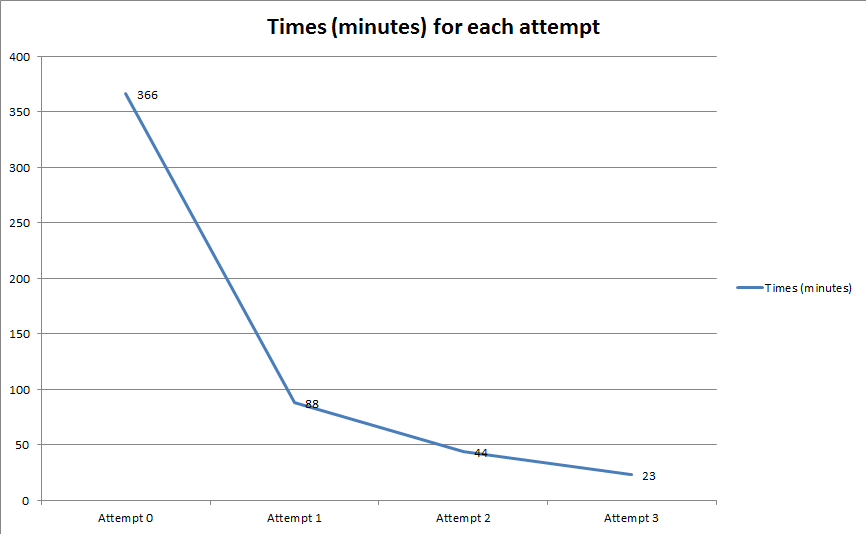
\includegraphics[scale=0.65]{./media/MyData_Times.png}
\caption{The times I took for each attempt as a line graph --- the huge drop from \AZ\ to \AO\
  suggests that analyses of this dataset might not be very effective.}
\label{figure:mytimes}
\end{figure}

This dataset might be much more difficult to analyse, due to the differences
between each data point being quite large and unpredictable.
This was due to spending a long time thinking, learning and debugging in \AZ,
whilst being able to effectively employ this knowledge in \AO.

\begin{table}[ht!]
\centering
\begin{tabular}{|c|c|c|c|}
\hline
{\bf Model} &  $a$ & $b$ & $c$ \\
\hline
$m_1$ & 365.988 & 2.53243 & -21.1487 \\
\hline
$m_2$ & 365.933 & 2.10872 & 5.5325 \\
\hline
$m_3$ & 365.833 & 1.66211 & 25.3253 \\
\hline
\end{tabular}
\caption{Parameters of the best fits for each of the models for the my data's
  time per attempt.}
\label{table:mytimes:abc}
\end{table}

\begin{figure}[ht!]
\centering
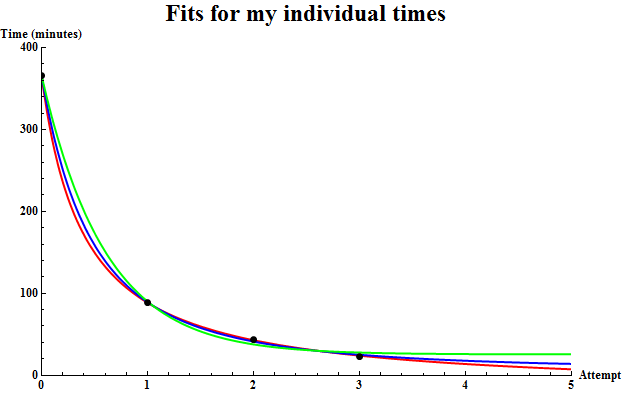
\includegraphics[scale=0.35,angle=90]{./media/MyTimesGraph.png}
\caption{The graph of models for the time taken in minutes for me to complete the programming tasks
	during my attempts. The key is as follows:
		 red is $m_1$,
		 blue is $m_2$,
		 green is $m_3$.
}
	\label{figure:mytimes:abc}
\end{figure}

Again, we see that the parameters of $m_1$ have fallen below 0, suggesting that
$m_1$ is not tolerant to such unpredictable, huge jumps.
$m_2$ has a somewhat suspicious result --- 5 and a half minutes to complete this
problem seems too short.
$m_3$ is probably the most sensible model, by inspection.

\begin{table}[ht!]
\centering
\begin{tabular}{|c|c|c|c|}
\hline
{\bf Model} &  $a$ & $b$ & $c$ \\
\hline
$m_1$ & 1.64553 & 0.116261 & 3.31338 \\
\hline
$m_2$ & 3.66321 & 0.13148 & 6.43122 \\
\hline
$m_3$ & 8.15699 & 0.177838 & 7.62098 \\
\hline
\end{tabular}
\caption{Standard errors for the parameters of the best fits for each of the
  models for my data's time per attempt.}
\label{table:mytimes:abc:error}
\end{table}

The errors shown in Table \ref{table:mytimes:abc:error} disagree with my
rudimentary analysis, however.
$m_3$ appears to have suffered a lot of errors, especially in predicting $c$,
due to the huge jumps.
It also had a surprisingly large error in predicting $a$.

\begin{table}[ht!]
\centering
\begin{tabular}{|c|c|}
\hline
{\bf Model} & Sum of squares \\
\hline
$m_1$ & 2.707908\\
\hline
$m_2$ & 13.42355\\
\hline
$m_3$ & 66.56446\\
\hline
\end{tabular}
\caption{Sum of squares of the residuals for the best fits for each of the
  models for my data's time per attempt.}
\label{table:mytimes:abc:sumsquares}
\end{table}

Table \ref{table:mytimes:abc:sumsquares} further suggests that $m_3$ is
inappropriate, due to having a very large least sums of squares.
However, given the results that both $m_1$ and $m_2$ have shown and how they are
somewhat impossible, I feel that $m_3$'s parameters, though a poor fit are more
believable and useful that $m_1$ and $m_2$.\\
\\
I believe that overall, $m_3$ would have to be the appropriate model for my
learning process, due to it being sensible in terms of its results and also
approximating my final time required to complete the project much more closely
than $m_1$ and $m_2$.
It shows me taking a long time to, in an unguided fashion, perform a task.
Once I have successfully completed that task once, it shows how I can reproduce
that task in increasingly quicker times.
It was rather appropriate for my Waterfall-esque approach to completing this
task, in that it captured the idea of shortening the requirements and design
phases and simply performing the resulting code.
Furthermore, since I did not change algorithms and continually reduced my code I
think $m_3$ was the most appropriate model.
